\documentclass[../Main.tex]{subfiles}

\begin{document}

\IfFileExists{NewCommands.tex}       {% Add new commands here.
%
% Use "providecommand" instead of "newcommand" since we
% want to include this file in all subfiles, and if we
% used newcommand it would report the error
% "Command xxx already defined"
%
%
\providecommand{\dmOT}{\Delta m^2_{\rm 12}}
\providecommand{\dmsolar}{\Delta m^2_{\rm solar}}
\providecommand{\dmatm}{\Delta m^2_{\rm atm}}
\providecommand{\dmTT}{\Delta m^2_{\rm atm}}
\providecommand{\dmsq}[1]{\Delta m^{2}_{#1}}
\providecommand{\thatm}{\Delta m^2_{\rm atm}}
\providecommand{\thTT}{\theta_{\rm 23}}
\providecommand{\sinsq}[1]{\sin^{2}(\theta_{#1})}
\providecommand{\sinsqOT}{\sin^{2}(\theta_{\rm 12})}
\providecommand{\sinsqsolar}{\sin^{2}(\theta_{\rm solar})}
\providecommand{\sinsqTT}{\sin^{2}(\theta_{\rm 23})}
\providecommand{\sinsqTwoTT}{\sin^{2}(2\theta_{\rm 23})}
\providecommand{\dcp}{\delta_{\rm CP}}

\providecommand{\gsim}{\gtrsim}
\providecommand{\lsim}{\lesssim}
\providecommand{\Enu}{\rm{E}_\nu}
\providecommand{\Emu}{\rm{E}_\mu}
\providecommand{\Ecasc}{\rm{E}_{\rm casc}}
\providecommand{\Lmu}{\rm{L}_\mu}
\providecommand{\Lnu}{\rm{L}_\nu}
\providecommand{\Thetamu}{\theta_\mu}
\providecommand{\cosThetamu}{\cos{\theta_\mu}}
\providecommand{\cosThetanu}{\cos{\theta_\nu}}
\providecommand{\Thetanu}{\theta_\nu}
\providecommand{\nue}{\nu_{\rm e}}
\providecommand{\numu}{\nu_\mu}
\providecommand{\nutau}{\nu_\tau}

\providecommand{\ket}[1]{|#1\rangle}

\providecommand{\ue}[1]{|U_{e #1}|}
\providecommand{\umu}[1]{|U_{\mu #1}|}
\providecommand{\utau}[1]{|U_{\tau #1}|}
\providecommand{\uesq}[1]{|U_{e #1}|^{2}}
\providecommand{\umusq}[1]{|U_{\mu #1}|^{2}}
\providecommand{\utausq}[1]{|U_{\tau #1}|^{2}}

\providecommand{\Nch}{${\rm N}_{\rm ch}\,$}
\providecommand{\Ndir}{${\rm N}_{\rm dir}\,$}
\providecommand{\Nstr}{${\rm N}_{\rm str}\,$}
\providecommand{\Aeff}{${\rm A}_{\rm eff}\,$}
\providecommand{\Veff}{${\rm V}_{\rm eff}\,$}
\providecommand{\VeffNS}{${\rm V}_{\rm eff}$}

\providecommand{\pe}{$p.e.$ }
}       {}
\IfFileExists{../NewCommands.tex}    {% Add new commands here.
%
% Use "providecommand" instead of "newcommand" since we
% want to include this file in all subfiles, and if we
% used newcommand it would report the error
% "Command xxx already defined"
%
%
\providecommand{\dmOT}{\Delta m^2_{\rm 12}}
\providecommand{\dmsolar}{\Delta m^2_{\rm solar}}
\providecommand{\dmatm}{\Delta m^2_{\rm atm}}
\providecommand{\dmTT}{\Delta m^2_{\rm atm}}
\providecommand{\dmsq}[1]{\Delta m^{2}_{#1}}
\providecommand{\thatm}{\Delta m^2_{\rm atm}}
\providecommand{\thTT}{\theta_{\rm 23}}
\providecommand{\sinsq}[1]{\sin^{2}(\theta_{#1})}
\providecommand{\sinsqOT}{\sin^{2}(\theta_{\rm 12})}
\providecommand{\sinsqsolar}{\sin^{2}(\theta_{\rm solar})}
\providecommand{\sinsqTT}{\sin^{2}(\theta_{\rm 23})}
\providecommand{\sinsqTwoTT}{\sin^{2}(2\theta_{\rm 23})}
\providecommand{\dcp}{\delta_{\rm CP}}

\providecommand{\gsim}{\gtrsim}
\providecommand{\lsim}{\lesssim}
\providecommand{\Enu}{\rm{E}_\nu}
\providecommand{\Emu}{\rm{E}_\mu}
\providecommand{\Ecasc}{\rm{E}_{\rm casc}}
\providecommand{\Lmu}{\rm{L}_\mu}
\providecommand{\Lnu}{\rm{L}_\nu}
\providecommand{\Thetamu}{\theta_\mu}
\providecommand{\cosThetamu}{\cos{\theta_\mu}}
\providecommand{\cosThetanu}{\cos{\theta_\nu}}
\providecommand{\Thetanu}{\theta_\nu}
\providecommand{\nue}{\nu_{\rm e}}
\providecommand{\numu}{\nu_\mu}
\providecommand{\nutau}{\nu_\tau}

\providecommand{\ket}[1]{|#1\rangle}

\providecommand{\ue}[1]{|U_{e #1}|}
\providecommand{\umu}[1]{|U_{\mu #1}|}
\providecommand{\utau}[1]{|U_{\tau #1}|}
\providecommand{\uesq}[1]{|U_{e #1}|^{2}}
\providecommand{\umusq}[1]{|U_{\mu #1}|^{2}}
\providecommand{\utausq}[1]{|U_{\tau #1}|^{2}}

\providecommand{\Nch}{${\rm N}_{\rm ch}\,$}
\providecommand{\Ndir}{${\rm N}_{\rm dir}\,$}
\providecommand{\Nstr}{${\rm N}_{\rm str}\,$}
\providecommand{\Aeff}{${\rm A}_{\rm eff}\,$}
\providecommand{\Veff}{${\rm V}_{\rm eff}\,$}
\providecommand{\VeffNS}{${\rm V}_{\rm eff}$}

\providecommand{\pe}{$p.e.$ }
}    {}
\IfFileExists{../../NewCommands.tex} {% Add new commands here.
%
% Use "providecommand" instead of "newcommand" since we
% want to include this file in all subfiles, and if we
% used newcommand it would report the error
% "Command xxx already defined"
%
%
\providecommand{\dmOT}{\Delta m^2_{\rm 12}}
\providecommand{\dmsolar}{\Delta m^2_{\rm solar}}
\providecommand{\dmatm}{\Delta m^2_{\rm atm}}
\providecommand{\dmTT}{\Delta m^2_{\rm atm}}
\providecommand{\dmsq}[1]{\Delta m^{2}_{#1}}
\providecommand{\thatm}{\Delta m^2_{\rm atm}}
\providecommand{\thTT}{\theta_{\rm 23}}
\providecommand{\sinsq}[1]{\sin^{2}(\theta_{#1})}
\providecommand{\sinsqOT}{\sin^{2}(\theta_{\rm 12})}
\providecommand{\sinsqsolar}{\sin^{2}(\theta_{\rm solar})}
\providecommand{\sinsqTT}{\sin^{2}(\theta_{\rm 23})}
\providecommand{\sinsqTwoTT}{\sin^{2}(2\theta_{\rm 23})}
\providecommand{\dcp}{\delta_{\rm CP}}

\providecommand{\gsim}{\gtrsim}
\providecommand{\lsim}{\lesssim}
\providecommand{\Enu}{\rm{E}_\nu}
\providecommand{\Emu}{\rm{E}_\mu}
\providecommand{\Ecasc}{\rm{E}_{\rm casc}}
\providecommand{\Lmu}{\rm{L}_\mu}
\providecommand{\Lnu}{\rm{L}_\nu}
\providecommand{\Thetamu}{\theta_\mu}
\providecommand{\cosThetamu}{\cos{\theta_\mu}}
\providecommand{\cosThetanu}{\cos{\theta_\nu}}
\providecommand{\Thetanu}{\theta_\nu}
\providecommand{\nue}{\nu_{\rm e}}
\providecommand{\numu}{\nu_\mu}
\providecommand{\nutau}{\nu_\tau}

\providecommand{\ket}[1]{|#1\rangle}

\providecommand{\ue}[1]{|U_{e #1}|}
\providecommand{\umu}[1]{|U_{\mu #1}|}
\providecommand{\utau}[1]{|U_{\tau #1}|}
\providecommand{\uesq}[1]{|U_{e #1}|^{2}}
\providecommand{\umusq}[1]{|U_{\mu #1}|^{2}}
\providecommand{\utausq}[1]{|U_{\tau #1}|^{2}}

\providecommand{\Nch}{${\rm N}_{\rm ch}\,$}
\providecommand{\Ndir}{${\rm N}_{\rm dir}\,$}
\providecommand{\Nstr}{${\rm N}_{\rm str}\,$}
\providecommand{\Aeff}{${\rm A}_{\rm eff}\,$}
\providecommand{\Veff}{${\rm V}_{\rm eff}\,$}
\providecommand{\VeffNS}{${\rm V}_{\rm eff}$}

\providecommand{\pe}{$p.e.$ }
} {}


\graphicspath{{figures/}{DataProcessing/figures/}}


\section{Data Processing}\label{sec:DataProcessing}

Due to the limited satellite bandwidth at the South Pole, IceCube uses
both online trigger and filter algorithms to reduce the rate
before any data is sent to the North. Once in the North, there is a
common processing on the data executed en masse to further reject background
events and reduce the data at a central site to a size that is approximately
manageable by specific analyzers and local research institutions. The
online collection and filtering done at the South Pole will be
reviewed in Sec.~\ref{sec:OnlineDataCollection}, the central offline
processing will be reviewed in Sec.~\ref{sec:L3Filter}, and a suite of
other topoligical algorithms customarily used at higher cut levels
will be described in Sec.~\ref{sec:OtherTopoVariables}.

\begin{figure}[bth!]
\centering
%\includegraphics[scale=0.4]{figures/Online_IceCube_data_processing_flow_chart.pdf}
\includegraphics[scale=0.4]{Online_IceCube_data_processing_flow_chart.pdf}
\caption{\label{fig:DataFlowChart} Should we include, an obviously
  nicer, flow chart of data collection? More simple? Redundant because
it'll be in the IceCube Detector paper?}
\end{figure}

\subsection{DeepCore Fiducial and Veto
  Regions}\label{sec:FiducialVetoRegions}

Due to a staggered deployment season for instrumentation at the South
Pole and adaptations to new physics opportunities, the fiducial and
veto definitions related to the DeepCore volume were modified in each
of the IC79, IC86-1, IC86-2, and IC86-3 data taking seasons. The
fiducial region in each season is an amalgam of the deepest DOMs on
the standard IceCube strings and the DeepCore-specific strings. As a reminder
the IceCube string DOM-DOM spacing is 17 m over the entire deployed
depth of 1450 to 2450~km, whereas the DeepCore instrumentation has
two distinct groupings of DOMs. At depths between 2100 and 2450~m
there are 50 DOMs with a 7~m DOM-DOM spacing. There is a gap in
instrumentation from 1850 to 2100~m which includes a region where the photon scattering and
absorption is higher than in the deeper and shallower
regions. The uppermost 10 DOMs on each DeepCore string are deployed
between 1750 to 1850~m with a DOM-DOM spacing of 10~m and constitute a
veto `plug' which enhances the ability to reject highly vertically
cosmic ray muon background. The fiducial and veto regions are a
combination of DOMs on both the standard IceCube and DeepCore-specific
strings.

\begin{figure}
\centering
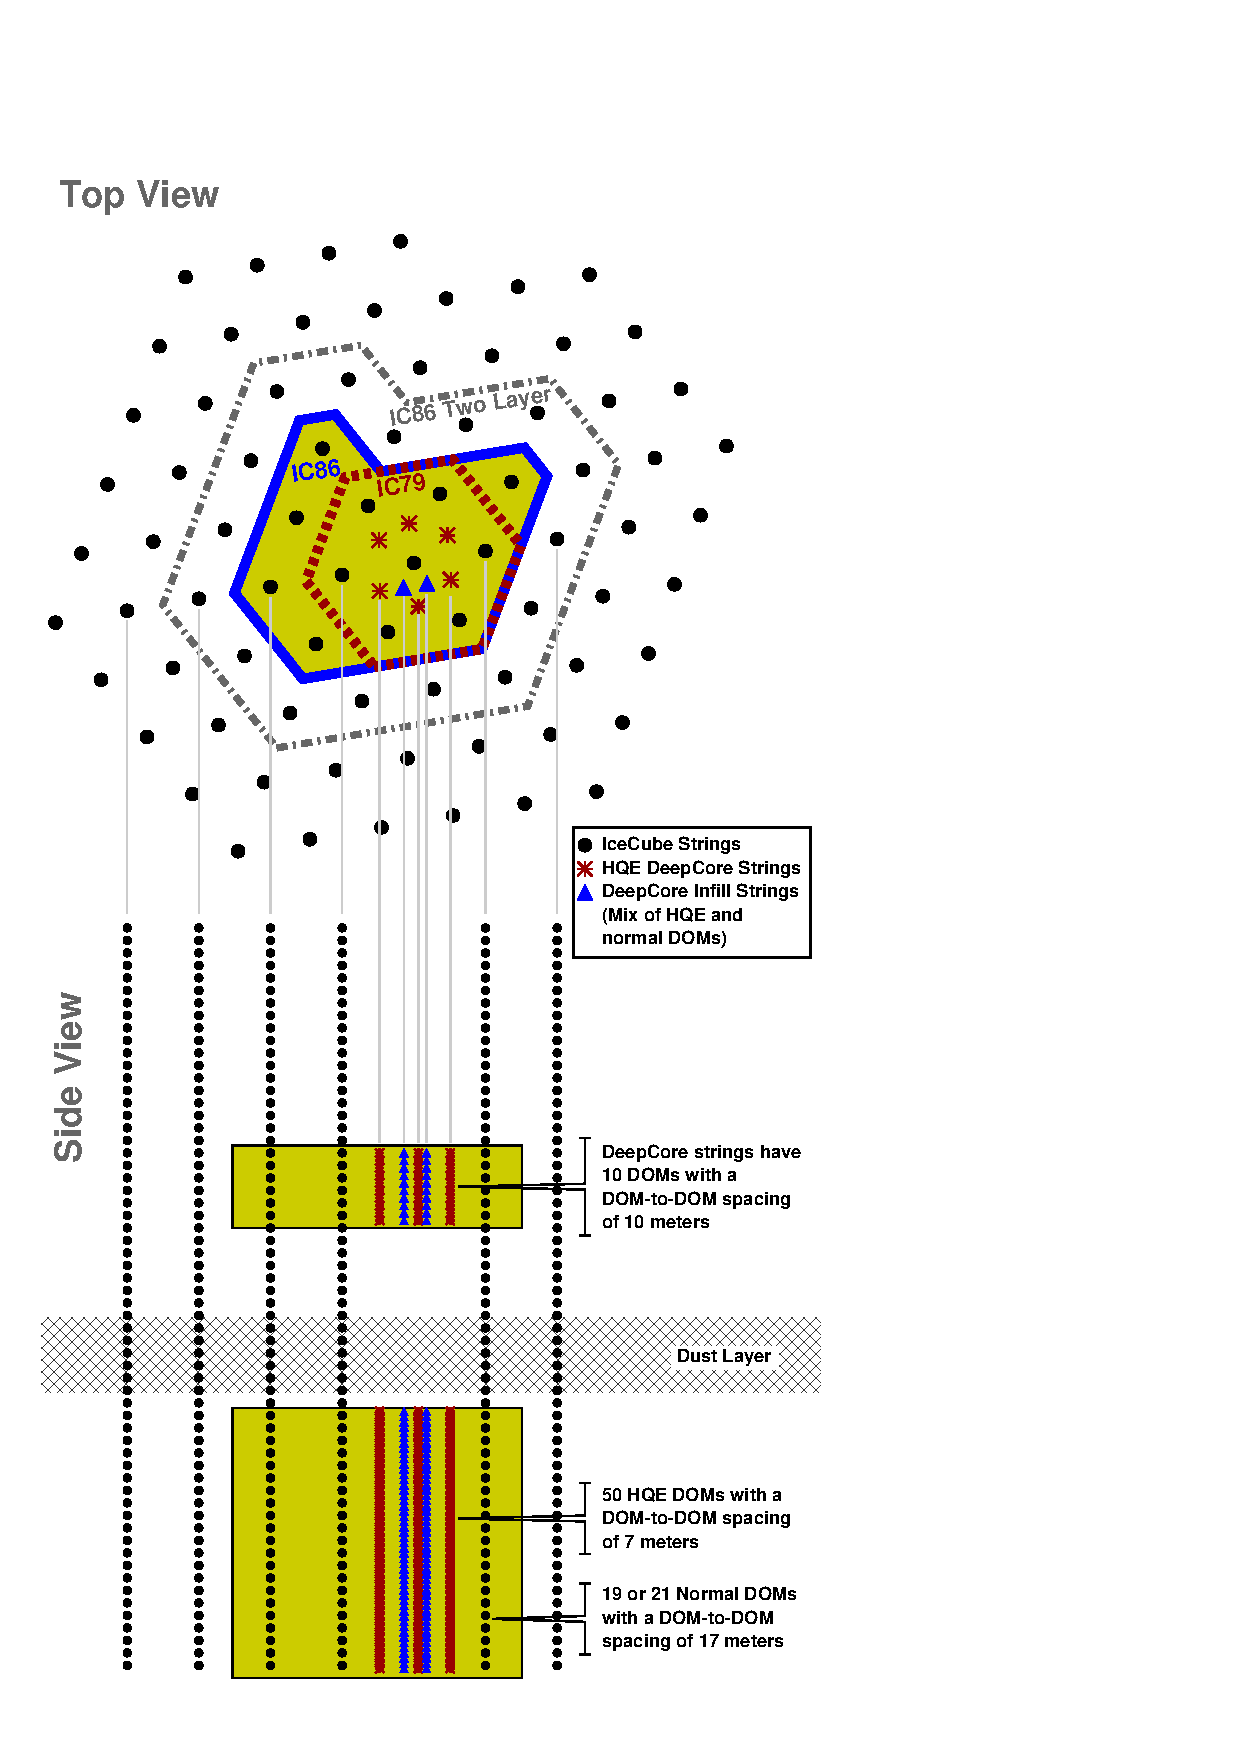
\includegraphics[scale=0.6]{IC86EDC_DeepCoreDiagram.pdf}
\caption{\label{fig:IC86EDCDiagram} Diagram of the IceCube-DeepCore
  fiducial and veto regions. The shaded region within the red dashed
  line is the trigger and online filter fiducial volume for the IC79
  configuration. The shaded region within the blue line is a
  trigger and fiducial volume for the IC86 configurations, which includes
  the 2 infill strings (blue triangles). For IC86-2
  a second low-energy filter was introduced using the shaded region
  within the blue line as the trigger volume, but defining the filter fiducial
  volume as everything within a 2-layer (grey dot-dash line) instead
  of 3-layer shell. The 2-layer veto has so far only been used in
  searches for transient astrophysical neutrino emission. 
}
\end{figure}

In IC79 the DeepCore fiducial volume includes the bottom 19 DOMs
(41-60) on the 7 central IceCube strings (26, 27, 35, 36, 37,
and 45) as well as the bottom 50 DOMs (10-60) on the 6 deployed DeepCore-specific strings
(81-86). This definition provided 3 layers of standard IceCube strings
for a veto volume which surrounds the fiducial volume. 

In IC86-1 the
last 7 strings for the IceCube array were installed: 5 standard
IceCube strings and 2 DeepCore infill strings. The two infill strings
have the same DOM-DOM spacing as the other 6 DeepCore strings, but are
composed of an admixture of both HQE and normal QE DOMs. With the
completion of the detector, the veto volume still consisted of 3
concentric layers of IceCube strings, but the fiducial region was
expanded, as shown in Fig.~\ref{fig:IC86EDCDiagram}. Also, the DOMs on
the IceCube strings for inclusion in the DeepCore SMT3 and online
fiducial volume was redefined from using the bottom 19 DOMs to include
the bottom 21 DOMs (39-60). 

For IC86-2 an additional
filter was introducted using the same trigger volume as that of
IC86-1, but using a 2-layer veto shell instead of 3-layer shell. 

\subsection{Online Triggering and
  Filtering}\label{sec:OnlineDataCollection}

A detailed description of the IceCube-DeepCore specific
triggering and filtering can be found in
\cite{Collaboration:2011ym}. Briefly, the dedicated low-energy trigger
requires three IceCube-DeepCore fiducial DOMs be in hard local
coincidence (HLC) within 2.5~$\mu$sec; commonly known as simple
multiplicity trigger 3 (SMT3). The trigger used the same criteria from
IC79 until IC86-4, i.e. the most recent run configuration at time of
this publication, changing only as a result of additional DOM deployment between
the IC79 and IC86-1 seasons as well as the online filter has undergone minor changes in the implementation
over the same period. The trigger rate as a function of time is shown
in Fig.~\ref{fig:DCTriggerFilterRate}.

\begin{figure}
\centering
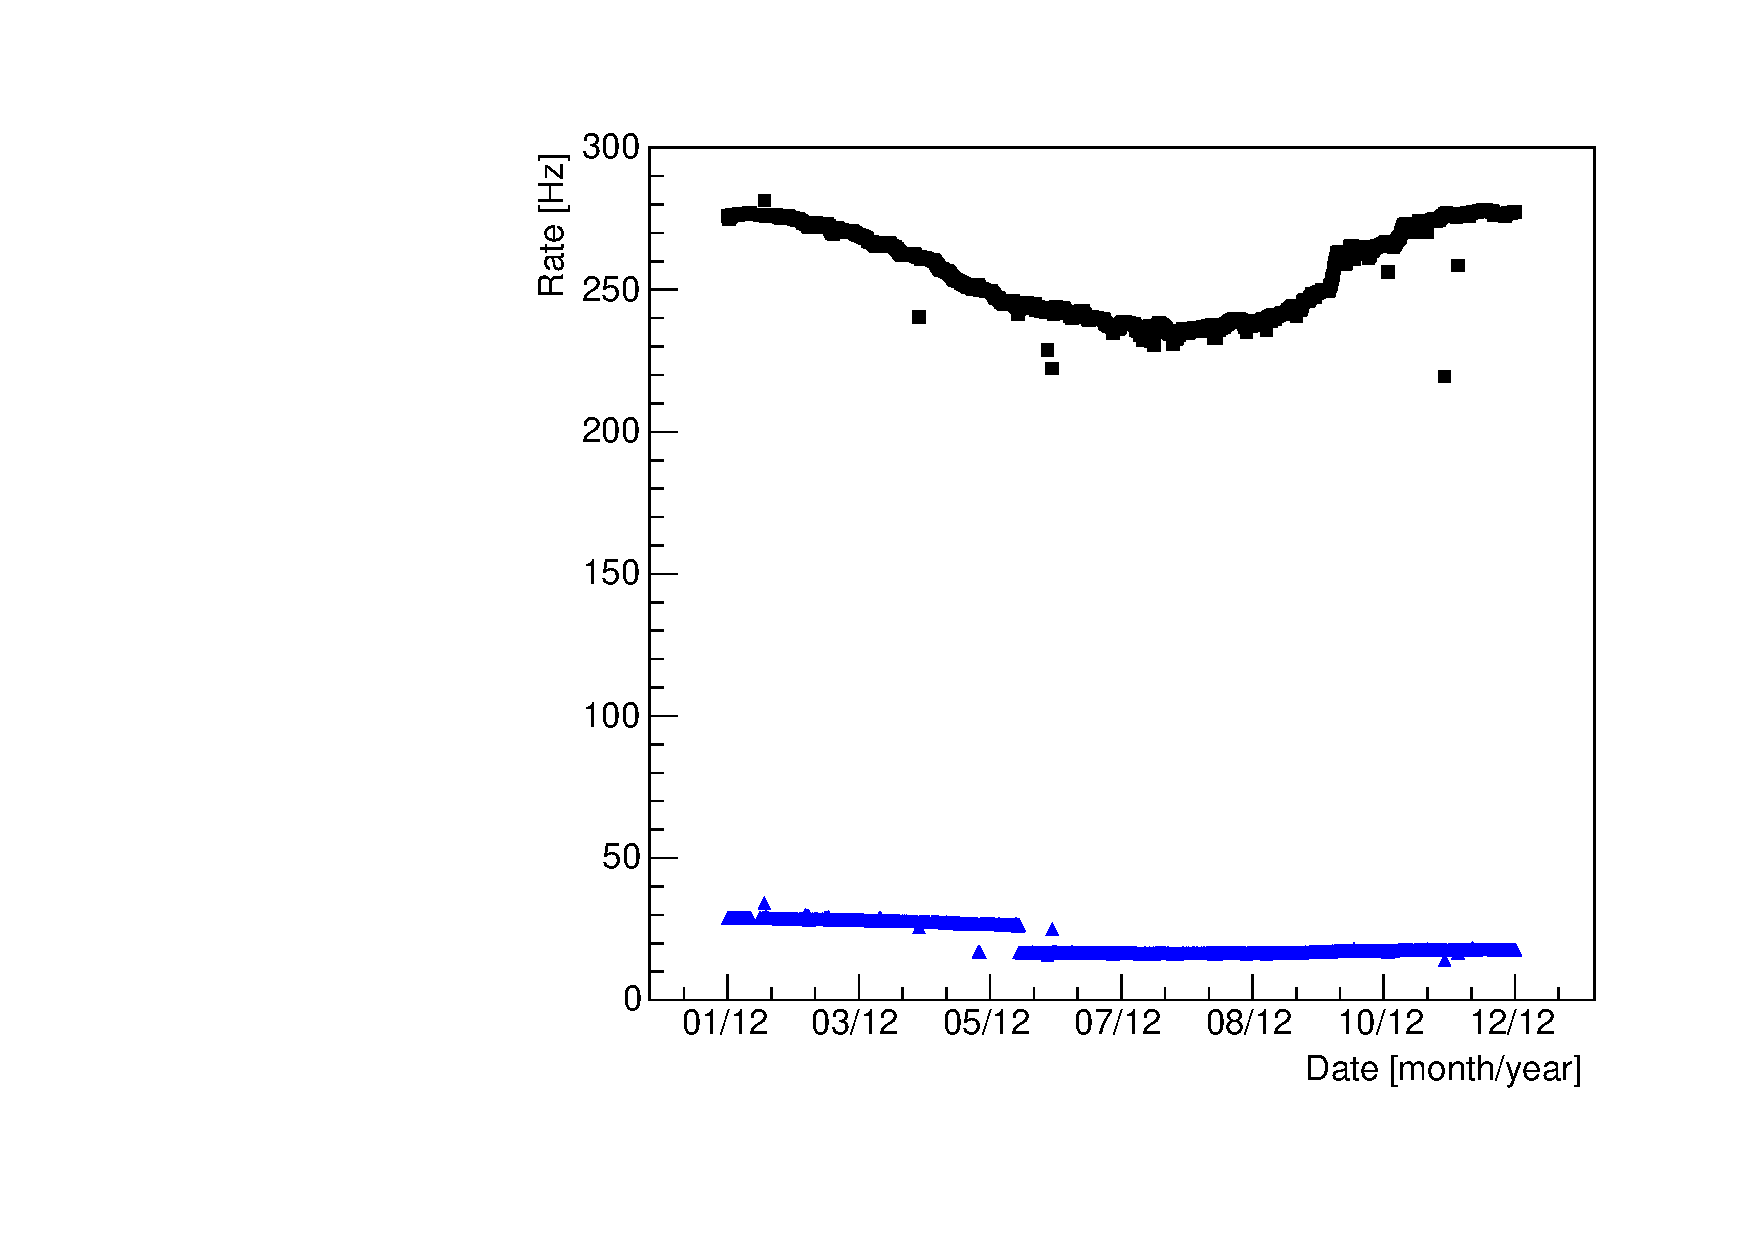
\includegraphics[scale=0.4]{DCTriggerFilterRate2012.pdf}
\caption{\label{fig:DCTriggerFilterRate} The dedicated DeepCore trigger (SMT3)
  rate (black squares) and online filter rate (blue triangles) as a function of time for runs with a
  duration of 1.5-8 hours that passed monitoring and
  verification checks and classified as `good' runs. The rate changes due to seasonal
  variations in the atmosphere and is dominated by cosmic ray
  muons. The discrete `jump' in the filter rate on May 15, 2012
  relates to a change in settings for the IC86-2 run.}
\end{figure}

Besides the seasonal variation in trigger rate, there is also a
decrease in the year-to-year rate, which is most pronounced for the
earlier data taking seasons. The decrease closely follows a drop
in the DOM noise rates, discussed in Sec.~\textbf{[NOISE still to be
  added]}. 

The online DeepCore filter is designed to reject events that show clear
indication of a penetrating cosmic ray muon, and is run for every
SMT3. Using the hits in the DeepCore fiducial region a
center-of-gravity (CoG) is generated producing both an average
position ($\vec{r}$) and time ($t$). For each hit in the veto region a
speed is a calculated to the DeepCore CoG, and any event with more
than one CoG-veto pair having a speed between +0.25 m/ns and +0.4 m/ns
is rejected.

% run 120156 is the change to IC86-2

There is a discrete shift in the filter rate in 2012,
which coincides to a change from using the hardware launch time of
the DOM to using the extracted hits from the DOM \textbf{[n.b. Needs much
more, but to be done later]}.

\subsection{Offline Central Data Processing}\label{sec:L3Filter}

The intial central processing for the low-energy data stream
includes three common features:
\begin{itemize}
\item{Hit series cleaning}
\item{Pre-selection using 3 cleaning cuts to reject noise-only events}
\item{Straight cuts on 6 topological variables}
\end{itemize}

Events that pass the online DeepCore filter undergo the following
central data processing at UW-Madison. The data or simulation after
triggering is commonly known as `level 1' (L1), after online filtering is
`level 2' (L2), and after the central offline filtering is `level 3'
(L3).

\subsubsection{Hit Series Cleaning}\label{sec:HitSeriesCleaning}

The IceCube detector operates multiple triggers and reads out hits
from the whole detector, often including noise hits which are
unrelated to any physics interaction as well as hits from multiple
coincident physics interactions, e.g. penetrating cosmic ray muons
from two or more unrelated primary cosmic rays. In order to remove noise
hits, or separate physics hits from coincident particles, there is a suite of
hit `cleaning' alrogithms which are used in IceCube-DeepCore
analyses. Each algorithm takes a user-defined hit series and produce an
output hit series. It is common to use the output of one cleaning as
the input to another in series to produce multiple hit series
specialized for purity, efficiency, low scatter, etc...

Static Time Window (STW) - The algorithm selects all hits
within two separate time intervals preceding and following the time of
a trigger.

Dynamic Time Window (DTW) - Uses a pre-defined time interval
and produces a hit series with the highest concentration of hits
within that contiguous interval.

Classic Radius-Time (RT) - Each hit in the input series is compared to the rest of
the series and kept if it satisfies both a radial (R) and time (T)
window with a single neighboring hit. If a hit cannot satisfy the RT
condition, then it is rejected from the cleaned output
series. Because Classic RT removes hits from the input series which
fail the RT criteria, it has a higher efficiency for retaining phyics hits, but lower purity,
than the Seeded RT cleaning, which is detailed below. 

\textbf{[n.b. can two hits on the same DOM satisfy the RT 
condition? Must the hits be on another DOM? What happens with multiple
pulses in the FADC range from an HLC pair that are outside the time
criteria of the neighbour DOM, e.g. 79-55 (10,000 ns) and 79-56 (10,300
ns, 11,200ns, 11,700ns)?]}

Seeded Radius Time (Seeded RT) - The cleaning is similar to the
RT cleaning in that retained hits must satisfy a radius and time
criteria, but instead of comparing each hit (SLC and HLC) to every 
other hit in the series, seeded RT starts with a smaller seed hit
series. 

The most common seed option is `HLCCoreHits', which creates an initial seed
series of only HLC hits which themselves satisfy RT 
criteria, via the classic RT cleaning detailed above. At the next
iteration, any hit which satisfies the RT criteria to any of the seed
hits is added to the series. The process stops after a user defined
number of iterations or when no new hits are added to the seed
series.


% Taken from icetray-inspect of STTools
%The name of the procedure to use for determining the initial seed hits. The following values are possible: "AllHLCHits": All HLC hits will be used as seed hits. "AllCoreHits": All hits that have at least NHitsThreshold partner ST hits will be used as seed hits. "HLCCoreHits": Only HLC hits, that have a certain amount of partner ST HLC hits. If the AllowNoSeedHits parameter is set to ``false`` and the HLC core is empty, all HLC hits will be used as seed hits, and if no HLC hits are present at all, no output will get written to the frame. "HLCCOGSTHits": Hits which fulfill the ST conditions around the Center-of-Gravity of all HLC hits, are used as seed hits. "OMKeyHits": Select all hits as seed hits which belong to the OMs present in the configured (SeedOMKeyList) list of OMKey objects. "FirstOMKeyHits": Select hits as seed hits which belong to the OMs present in the configured (SeedOMKeyList) list of OMKey objects and are the first hits within the OM's hit series.

\textbf{Make a plot to describe STW and DTW. }

\subsubsection{Offline Pure-Noise Cleaning Cuts}\label{sec:L3Cleaning}

Many of the lowest multiplicity events that pass the DeepCore online filter
result from detector noise with no associated cosmic ray muon or
neutrino interaction.  These pure-noise events satisfy the trigger criteria of at least 3 HLC
hits on any of the DeepCore fiducial DOMs in 2.5~$\mu$sec and pass
the online filter because there are no hits in the outer IceCube veto
region that would identify it as an incoming cosmic ray
muon. Pure-noise triggers are unlikely to look like penetrating muons,
but they also do not produce hits which cluster in time and/or
space similar to low-energy neutrinos. Whereas the online filter
rejects events which look like muons, the cleaning cuts are designed
to reject events that do not look like neutrinos or muons,
i.e. pure-noise triggers.

Two of the three cleaning cuts designed to remove pure-noise events
use pulses only in the DeepCore fiducial region from cleaning algorithms
described in Sec.~\ref{sec:HitSeriesCleaning}, specifically a static
time window cleaning of
-5000~ns to +4000~ns (STW9000) followed by a dynamic time window cleaning of
300~ns (DTW300). Events which have more than 2 pulses and 2 \pe in
the STW9000\_DTW300 DeepCore fiducial hit series are kept.

The NoiseEngine algorithm\cite{LarsonMasters}, inspired by the TrackEngine muon trigger
algorithm\cite{diva2:328163}, uses the timing and location of the hits
to reject pure-noise events.\textbf{[Larson to write]}

\subsubsection{Shared variables for further cosmic muon reduction}\label{sec:L3Variables}

After the removal of events failing the pure-noise cleaning, the
data rate is $\mathcal{O}(10)$~Hz and dominated by cosmic ray muon
background. Due to the large data rate, we make straight cuts on the
following 6 non-computationally generated variables: 

% Pulses series is "SRTTWOfflinePulsesDC"
\textbf{Time Integrated Charge Ratio} - The variable `QR6' is the
ratio of the charge in the first 600~ns compared to the total
charge. Values close to one indicate more neutrino-like events, while
events with values closer to zero are more cosmic ray muon-like. To
minimize the impact of noise hits, the DeepCore common processing uses
`C2QR6' which is the same charge ratio, but with the first two hits
removed and also uses a SeededRT cleaned pulse series. Events pass which have a C2QR6 ratio $>0.4$.

\textbf{Total Charge in Upper Veto Region} - The variable `NAbove200'
is the total charge of the uncleaned pulses in the  -2000~ns
preceding the DeepCore trigger which are located in the upper regions
of the IceCube detector (z-position $>$ -200~m). Events with $<$~12~\pe in the upper veto region pass this cut.

% Pulses series is "SRTTWOfflinePulsesDC"
\textbf{Z-position of the First Hit} - The z-position of the first hit in a
pulse series. Events which have a first hit in SeededRT cleaned pulses
series at depths $<$~-120~m are kept. 

\textbf{Charge Ratio Between Veto and Fiducial Region} - Ratio of the
total charge of the SeededRT hits in the DeepCore veto region to the fiducial
region.  Events pass which have a $Q_{veto}/Q_{fiducial}<$~1.5.

% How do we consicely explain why events with > 1 causal p.e. 
% in the veto region pass the online filter?

\textbf{Total Charge of Causal Hits in the DeepCore Filter} - The
DeepCore filter outputs a veto decision as well as the intergrated
charge and total number of the uncleaned veto region hits which satisfy the
causality requirement.  Events pass which have $<$~7~\pe that
satisfy the DeepCore filter causality criteria. 

%https://docushare.icecube.wisc.edu/dsweb/Get/Document-62475/Martin_Wolf_RTVeto_LHVeto_Diffuse_PreMeeting_Aachen2012.pdf
%http://arxiv.org/pdf/1309.7007v2.pdf
\textbf{Radius-Time Veto} - Similar to the Radius-Time pulse cleaning,
the Radius-Time Veto (RTVeto) creates clusters of hits which satisfy
an RT-criteria, e.g. 250~m and 1~$\mu$s. The input pulses come from only
the veto region and have a time of 0~ns to 5000~ns before the DeepCore
trigger. Events are rejected depending on the total \pe of
the RTVeto cluster with the highest charge. For DeepCore common
processing in 2011, all events with an RTVeto cluster of $>4$~\pe were
rejected. The cut had the unintended consquence of also removing
$\mathcal{O}(100)$~GeV neutrinos for searches for transient astrophysical neutrino
emitters and atmospheric neutrino induced cascade measurements. The data
was reprocessed with a RTVeto criteria that is dependent on the total
charge in the DeepCore fiducial volume. Events must satisfy the
following criteria in order to pass:
\begin{itemize}
\item{ RTVeto250 $< 4$~\pe if DeepCore fiducial charge $<$ 100~\pe}
\item{ RTVeto250 $< 6$~\pe if 100~\pe $\leq$ DeepCore fiducial charge $<
    150$~\pe}
\item{ RTVeto250 $< 10$~\pe if 150~\pe $\leq$ DeepCore fiducial charge $<$
    200~\pe}
\item{ No RTVeto250 criteria if 200~\pe $\leq$ DeepCore fiducial charge}
\end{itemize}

Along with the modificaton of the RTVeto settings which were
re-appiled for the 2011 data, there is an
expanded branch of the common processing included for the 2012
seasons and beyond which is designed for better retention efficiency for cascade-like
neutrinos at $>\mathcal{O}(300)$~GeV. The same settings and variables
are used in the expanded bracnh except for C2QR6 and $Q_{veto}/Q_{fiducial}$. Events which
have a C2QR6 $>$~0.4 and $Q_{veto}/Q_{fiducial} >$~1.5 are kept, but
must also pass the rest of the aforementioned variables with the same
settings (NAbove200, RTVeto250, etc.).

\subsection{Common Topological Variables}\label{sec:OtherTopoVariables}

\begin{itemize}
\item{Location of first HLC DOM}

\item{Isolated pulses from ``blind'' directions (Corridor cut)}

\item{Isolated pulses in causal connection with the trigger (Sebastans L7, that shall finally be renamed)}
\end{itemize}

\subsection{Identification of ``direct'' Cherenkov light}
Consider a Cherenkov emitter with infinite range crossing the DeepCore volume. The light wavefront expands in the shape of a cone, which eventually meets a string of DOMs. When the cone passes by a string it projects a conic section in space and time: a hyperbola. A sketch of this is shown in Fig.\,\ref{fig:hyperbolas}. Particles with limited range will produce a section of the pattern shown.

\begin{figure}[!tbph]
  \centering
  \hspace*{\fill}
  \begin{subfigure}[b]{0.24\textwidth}
    \centering
    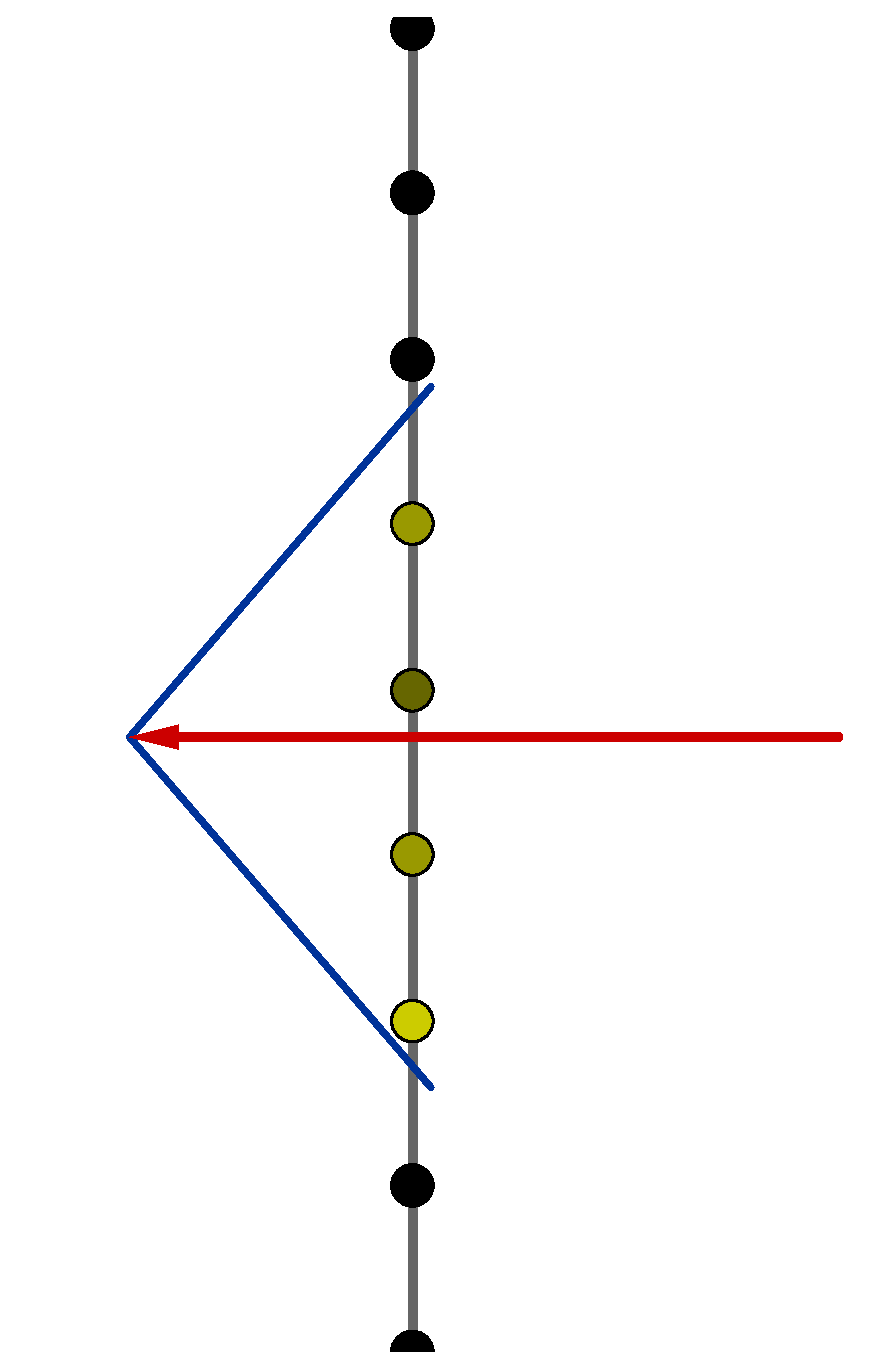
\includegraphics[width=\textwidth]{SANTA_1}
  \end{subfigure}\hfill
  \begin{subfigure}[b]{0.24\textwidth}
    \centering
    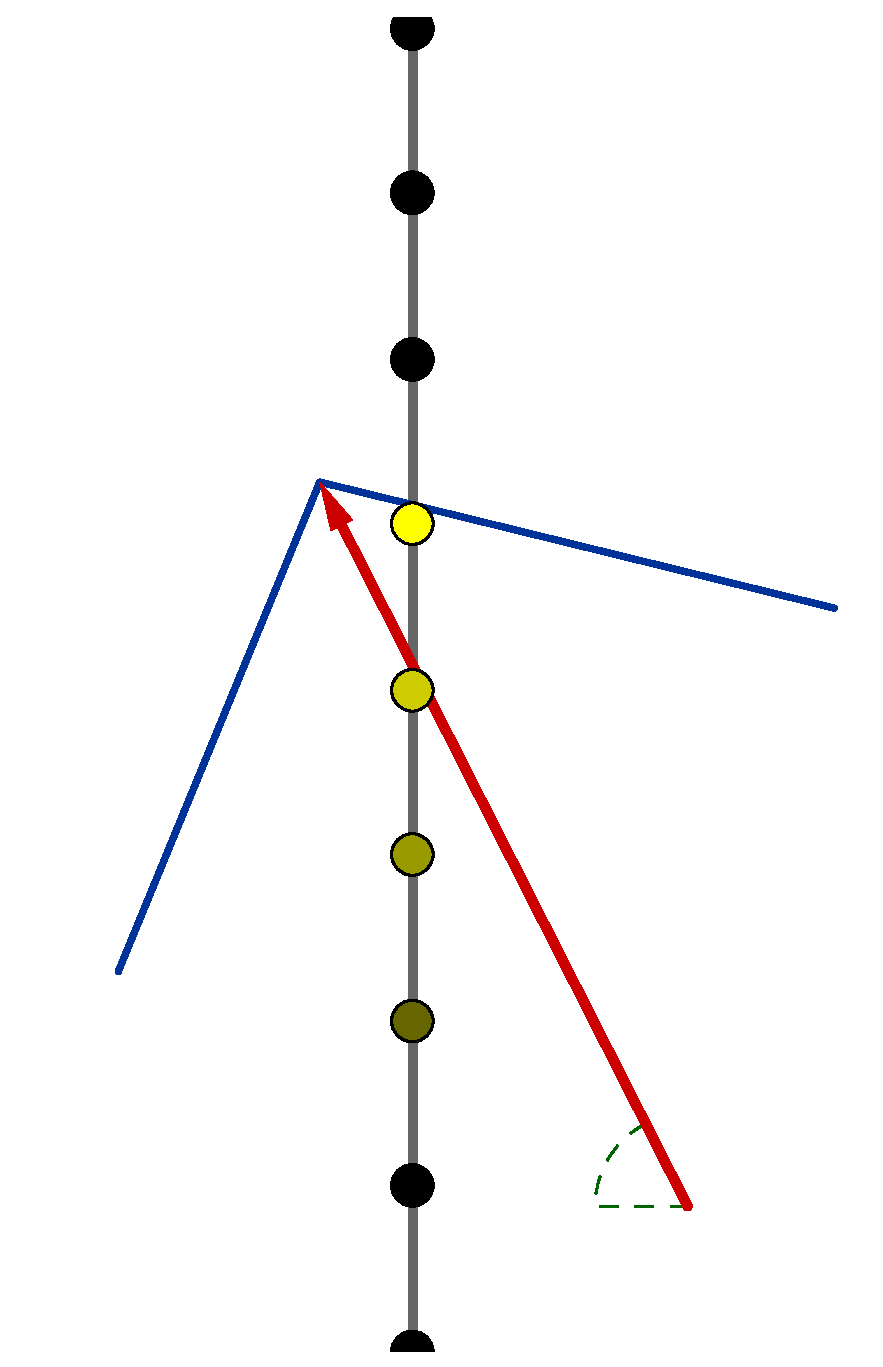
\includegraphics[width=\textwidth]{SANTA_2}
  \end{subfigure} \hspace*{\fill} \\
  \hspace*{\fill}
  \begin{subfigure}[b]{0.32\textwidth}
    \centering
    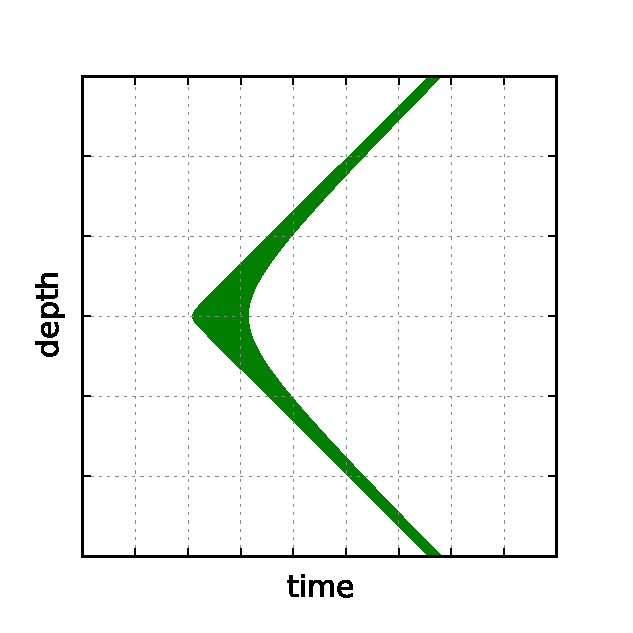
\includegraphics[width=\textwidth]{hyperbolas1}
  \end{subfigure}\hfill
  \begin{subfigure}[b]{0.32\textwidth}
    \centering
    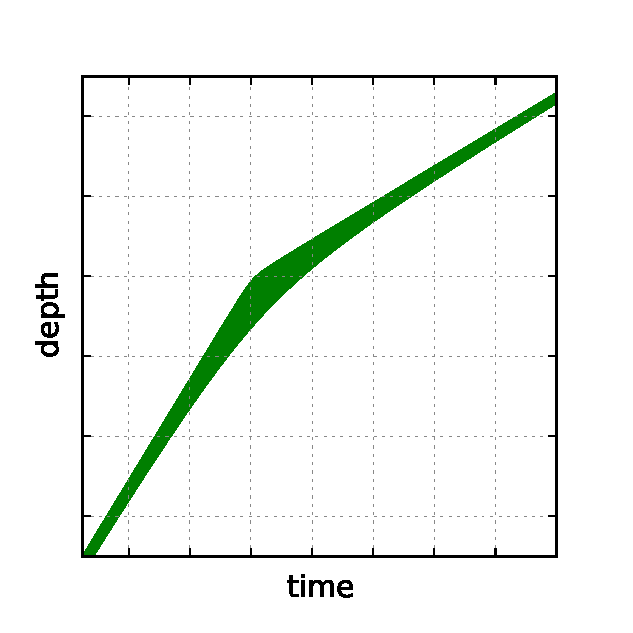
\includegraphics[width=\textwidth]{hyperbolas2}
  \end{subfigure}
  \hspace*{\fill}
  \caption[Hyperbolic patterns formed by Cherenkov light.]{Formation of hyperbolic patterns. Top: diagrams depicting the differences in arrival time of photons to the DOMs as a function of the orientation of the Cherenkov emitter (red). Dark yellow means early signals, bright yellow means late. Bottom: hyperbolas formed by the intersection of Cherenkov light with the detector's strings for the two geometric configurations on top and a distance between [0, 50]\,m between emitter and string.}
  \label{fig:hyperbolas}
\end{figure}

Since the pattern that direct photons create is known, it is possible to search for them based only on their time of arrival (TOA). This has to be done independently at each string, and is implemented on all the pulses detected by an algorithm that goes through the following steps:
\begin{enumerate}
\item Look for a string that has at least 3 DOMs with pulses, the minimum requirement to identify a hyperbola.
\item Characterize the signal of each DOM with the arrival time of the earliest pulse recorded, and integrate the charge of all the pulses recorded by the DOM.
\item Restrict the search to DOMs inside a time window of $[-1,+2]$\,$\mu$s around the median TOA for the string under consideration. The time window is approximately the one required for a particle to travel the elongation of a string.
\item Search for the DOM which has the largest integrated charge. This is an estimator of the point of closest approach and it is also the first DOM temporarily accepted; we call it DOM$_0$. Use this point as a reference to scan the string up and down searching for more DOMs.

\item From the starting point $t_0$, given by the earliest pulse at DOM$_0$, calculate a time window for testing the TOA of the pulse in the DOM above, DOM$_{+1}$. The time window is symmetric, and given by the time that a photon takes to travel between the two DOMs. It can be expressed as
  \begin{equation}
    \left[t_0 - \frac{d_\mathrm{0,+1}}{c_\mathrm{ice}} - t_\mathrm{delay}, t_0 + \frac{d_\mathrm{0,+1}}{c_\mathrm{ice}} + t_\mathrm{delay}\right]\,.
  \end{equation}
Here $d_\mathrm{0,+1}$ stands for the absolute distance between the two DOMs considered, 0 and +1, $c_\mathrm{ice}$ is the speed of light in ice, and the parameter $t_\mathrm{delay}$ determines how strict the selection is with regard to scattering effects. A value of 20\,ns for $t_\mathrm{delay}$ is used as a baseline. This step is repeated until one DOM is accepted. If none are, steps 6-8 are skipped.
%Any configuration of the light source will result in a time delay which is necessarily smaller than the one defined. 

\item Include the new DOM selected by the previous step in the search by defining a new time window for testing DOM$_{+2}$. While the lower limit is defined by the same conditions, the upper limit changes to reflect the newly acquired information. The time window is now given by
  \begin{equation}
    \left[t_1 - \frac{d_\mathrm{1,+2}}{c_\mathrm{ice}} - t_\mathrm{delay}, t_1 + \frac{d_\mathrm{1,+2}}{v_\mathrm{eff}} + t_\mathrm{delay}\right]\,,
    \label{eq:time_window2}
  \end{equation}
where $v_\mathrm{eff}$ defines an effective velocity for a photon that travels in between the two DOMs in question. This velocity is calculated using the last three DOMs that have been selected; the resulting possibilities are shown in Fig.\,\ref{fig:hits_cleaning}. The algorithm calculates all three effective velocities and takes the slowest one, allowing the largest time window possible.
\begin{figure}[tbph]
  \centering
  \hspace*{\fill}
  \begin{subfigure}[b]{0.37\textwidth}
    \centering
    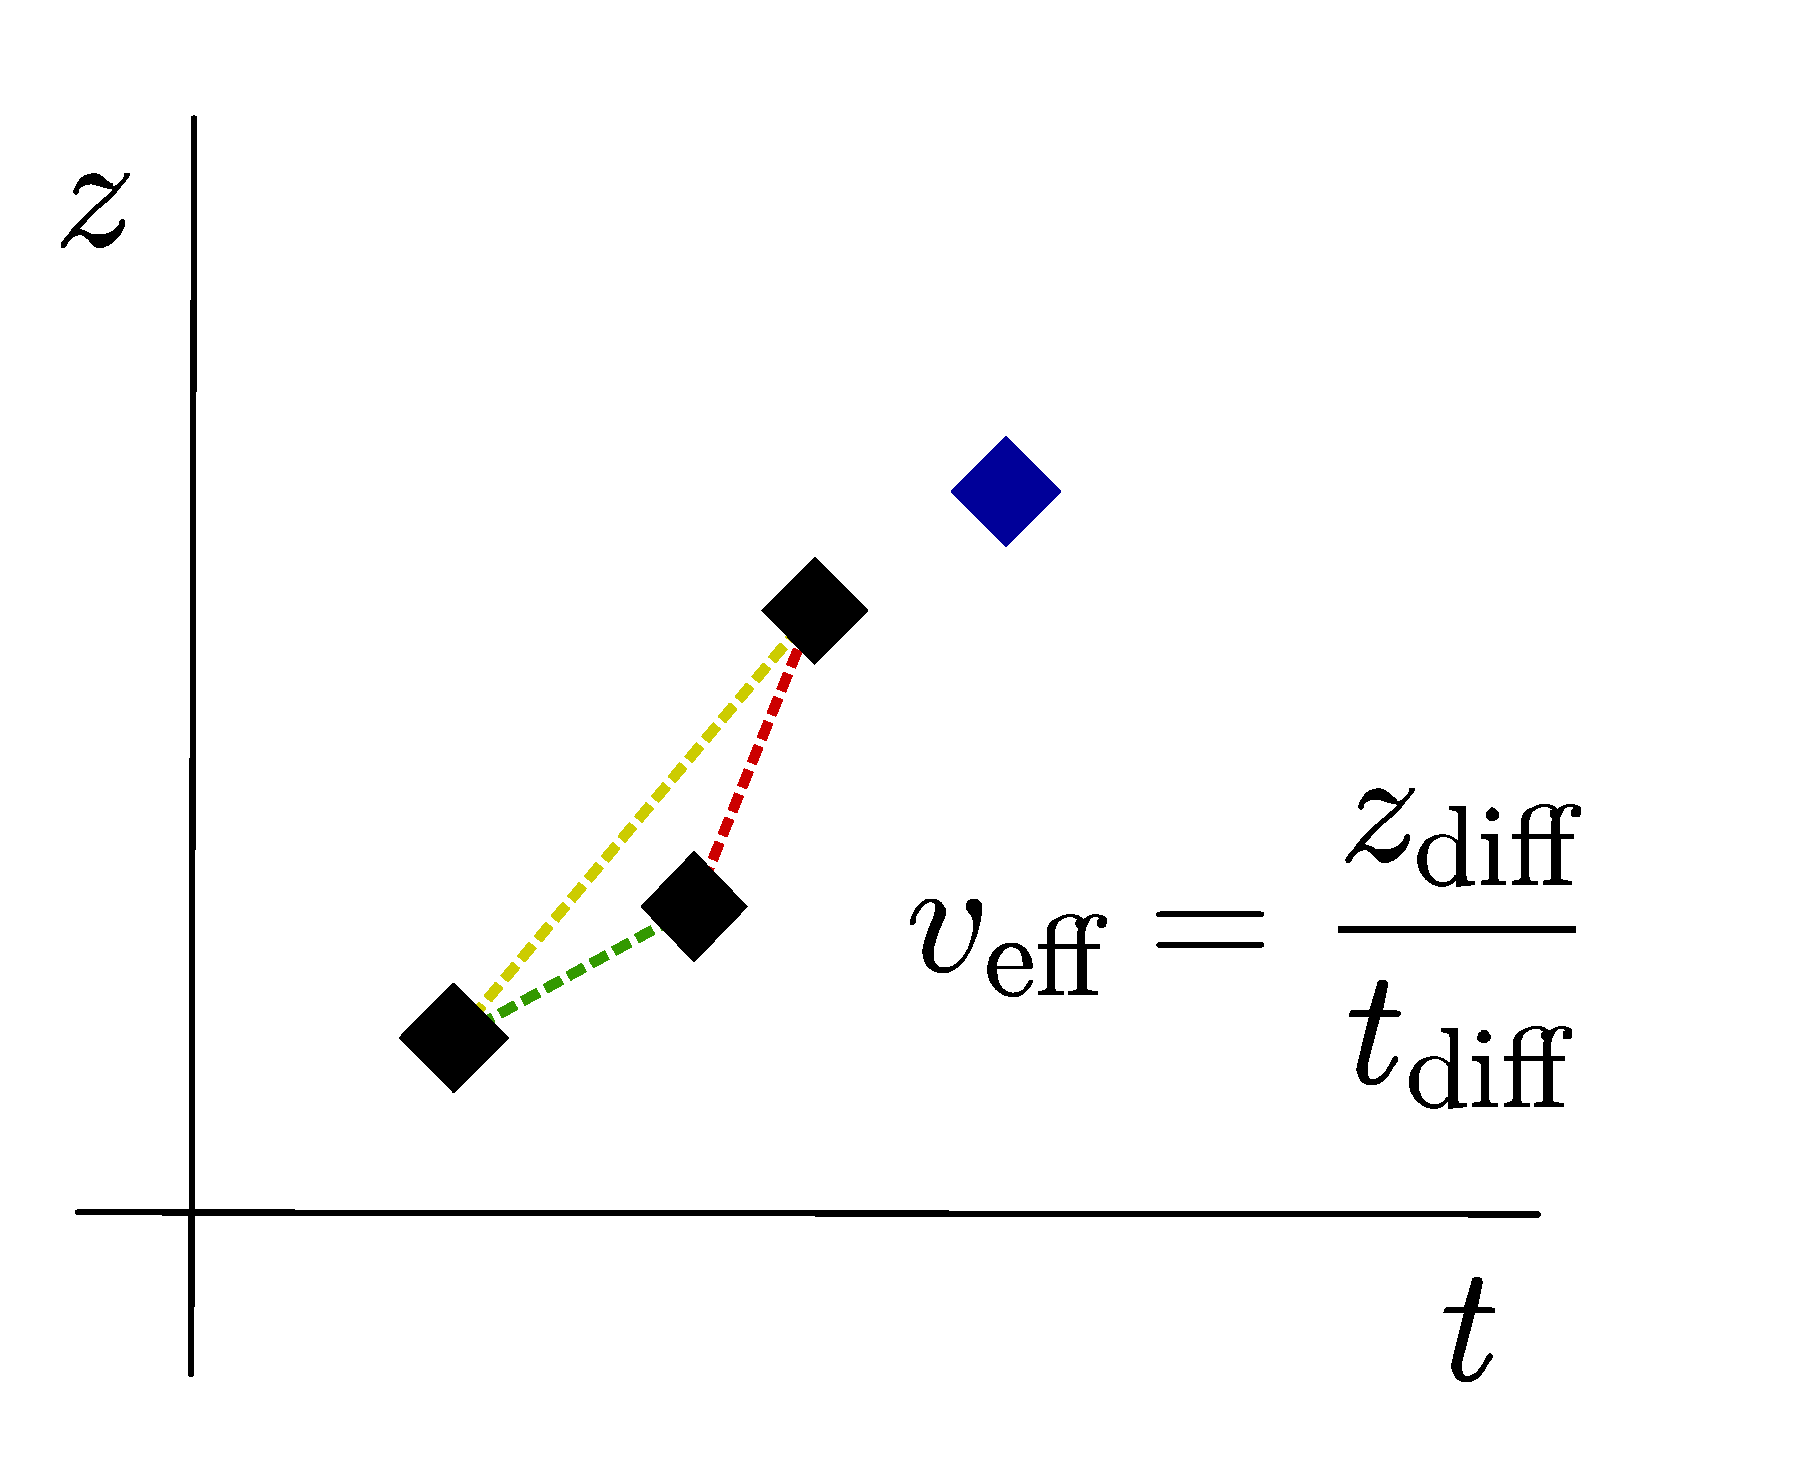
\includegraphics[width=\textwidth]{selection1}
    \caption{Possible $v_\mathrm{eff}$}
    \label{fig:cleaning1}
  \end{subfigure}\hfill
  \begin{subfigure}[b]{0.37\textwidth}
    \centering
    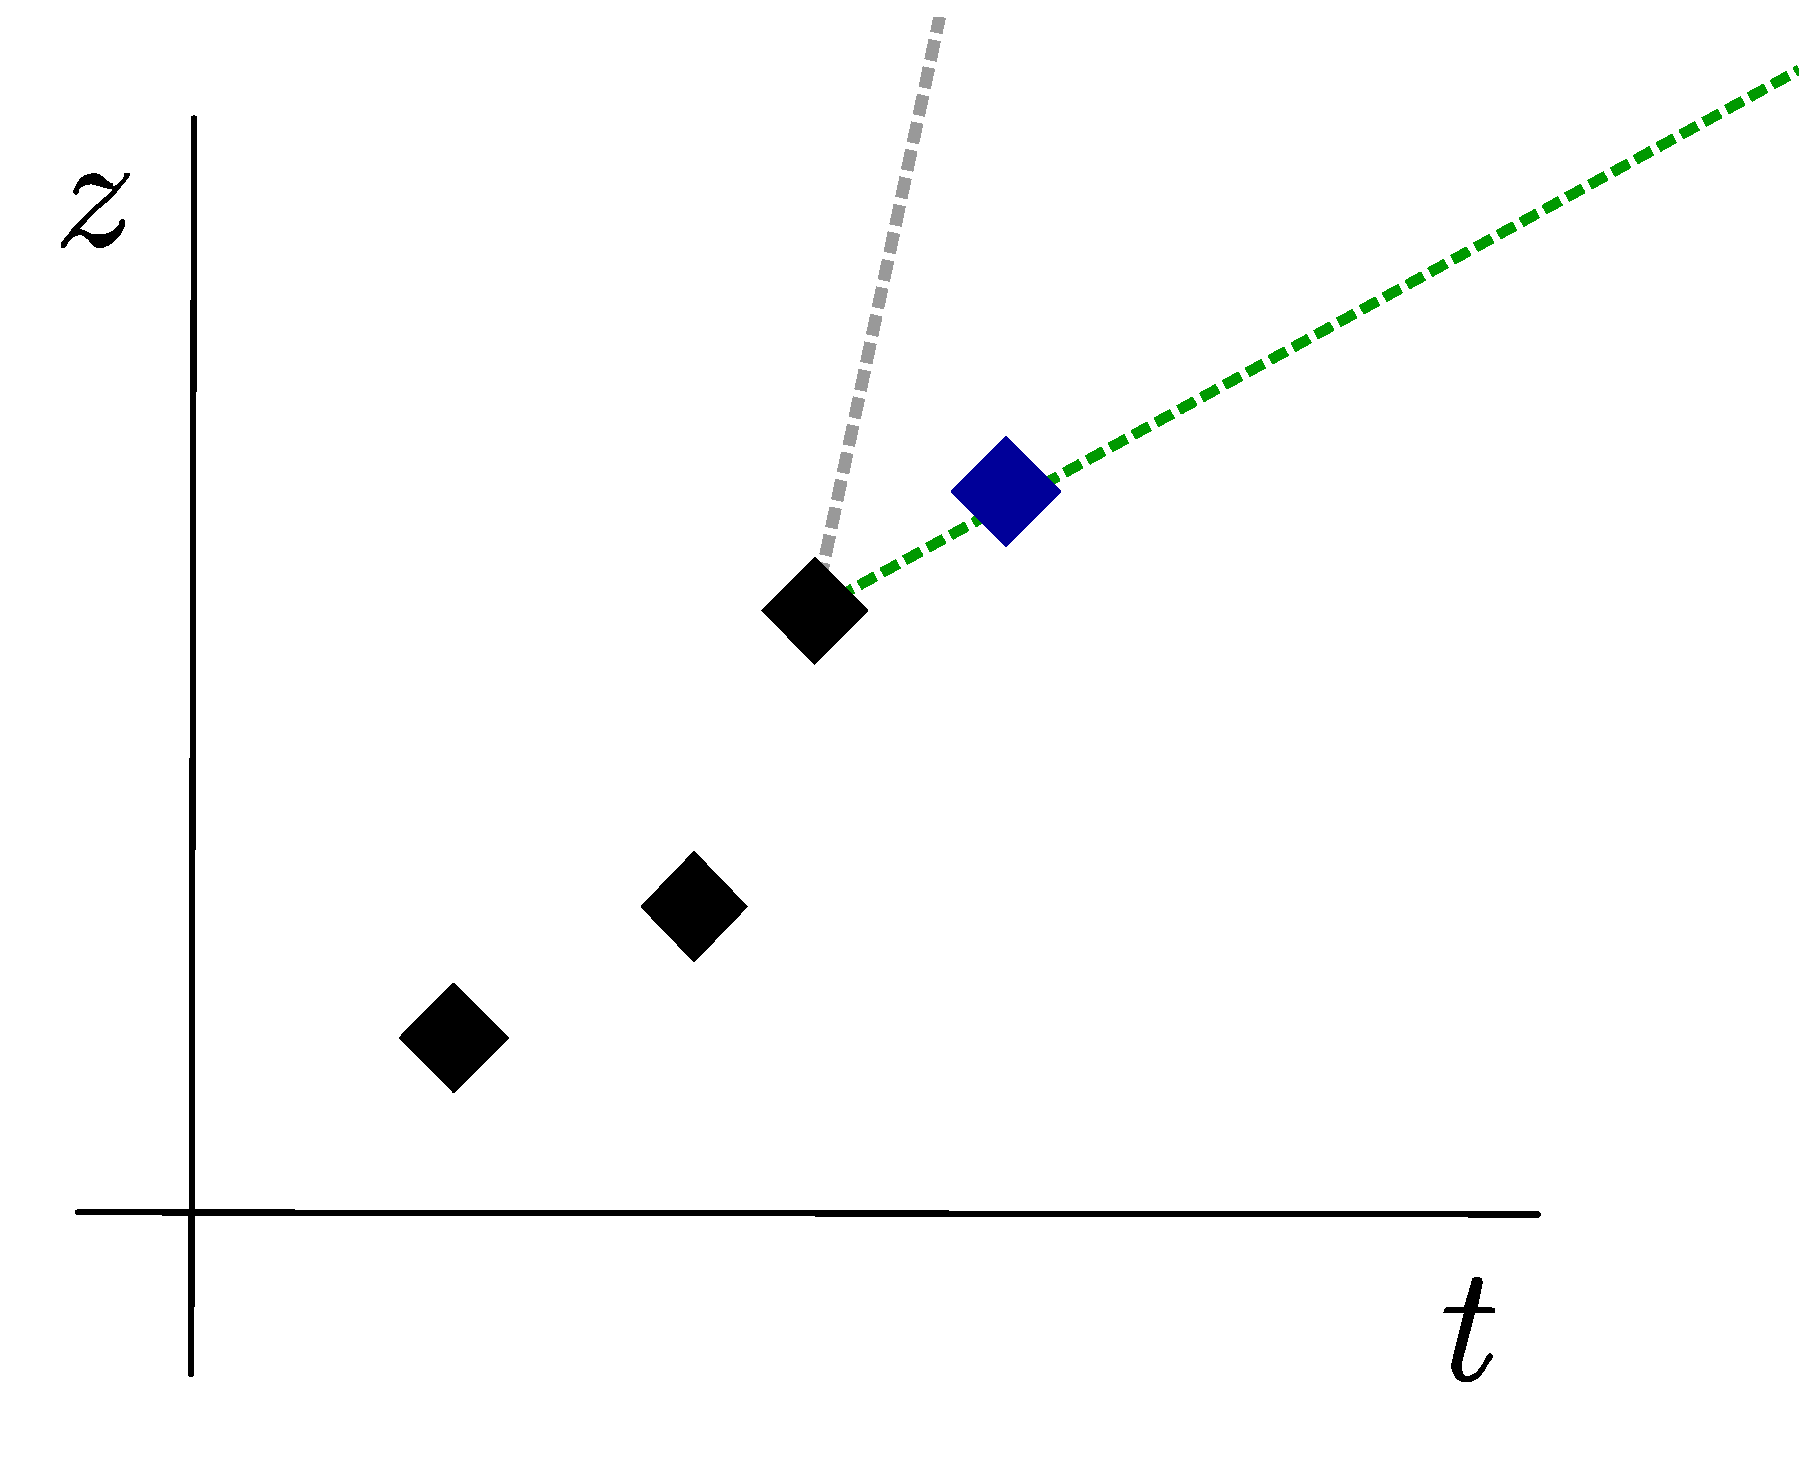
\includegraphics[width=\textwidth]{selection2}
    \caption{Slowest $v_\mathrm{eff}$}
    \label{fig:cleaning2}
  \end{subfigure}
  \hspace*{\fill}
  \caption[Criteria for selecting direct pulses.]{Criteria for selecting direct pulses. Markers represent pulses. Black pulses have been selected. The blue pulse is the one being tested. In (a) the three possible effective velocities given the pulses that have been selected are shown. In (b) the smallest effective velocity is applied (green line). The gray line is the earliest time of arrival allowed, as given by Eq.\,\ref{eq:time_window2}. In this example, the blue pulse would be taken.}
  \label{fig:hits_cleaning}
\end{figure}
\item Every time that a new DOM$_n$ is taken, check again if all previous DOMs still match the hyperbolic shape. Using DOM$_n$ and DOM$_0$ calculate an expected time of arrival for the signal of every intermediate DOM and allow a delay of $t_\mathrm{delay}/2$. If a DOM falls outside the window, remove it from the selection. Figure \ref{fig:hit_discarded} sketches a situation in which, depending on the $t_\mathrm{delay}$ used, the marked hit could be removed. This step allows for early photons to be used to remove scattered photons that might have been selected.

\begin{figure}[1.2][tbh]
  \centering
  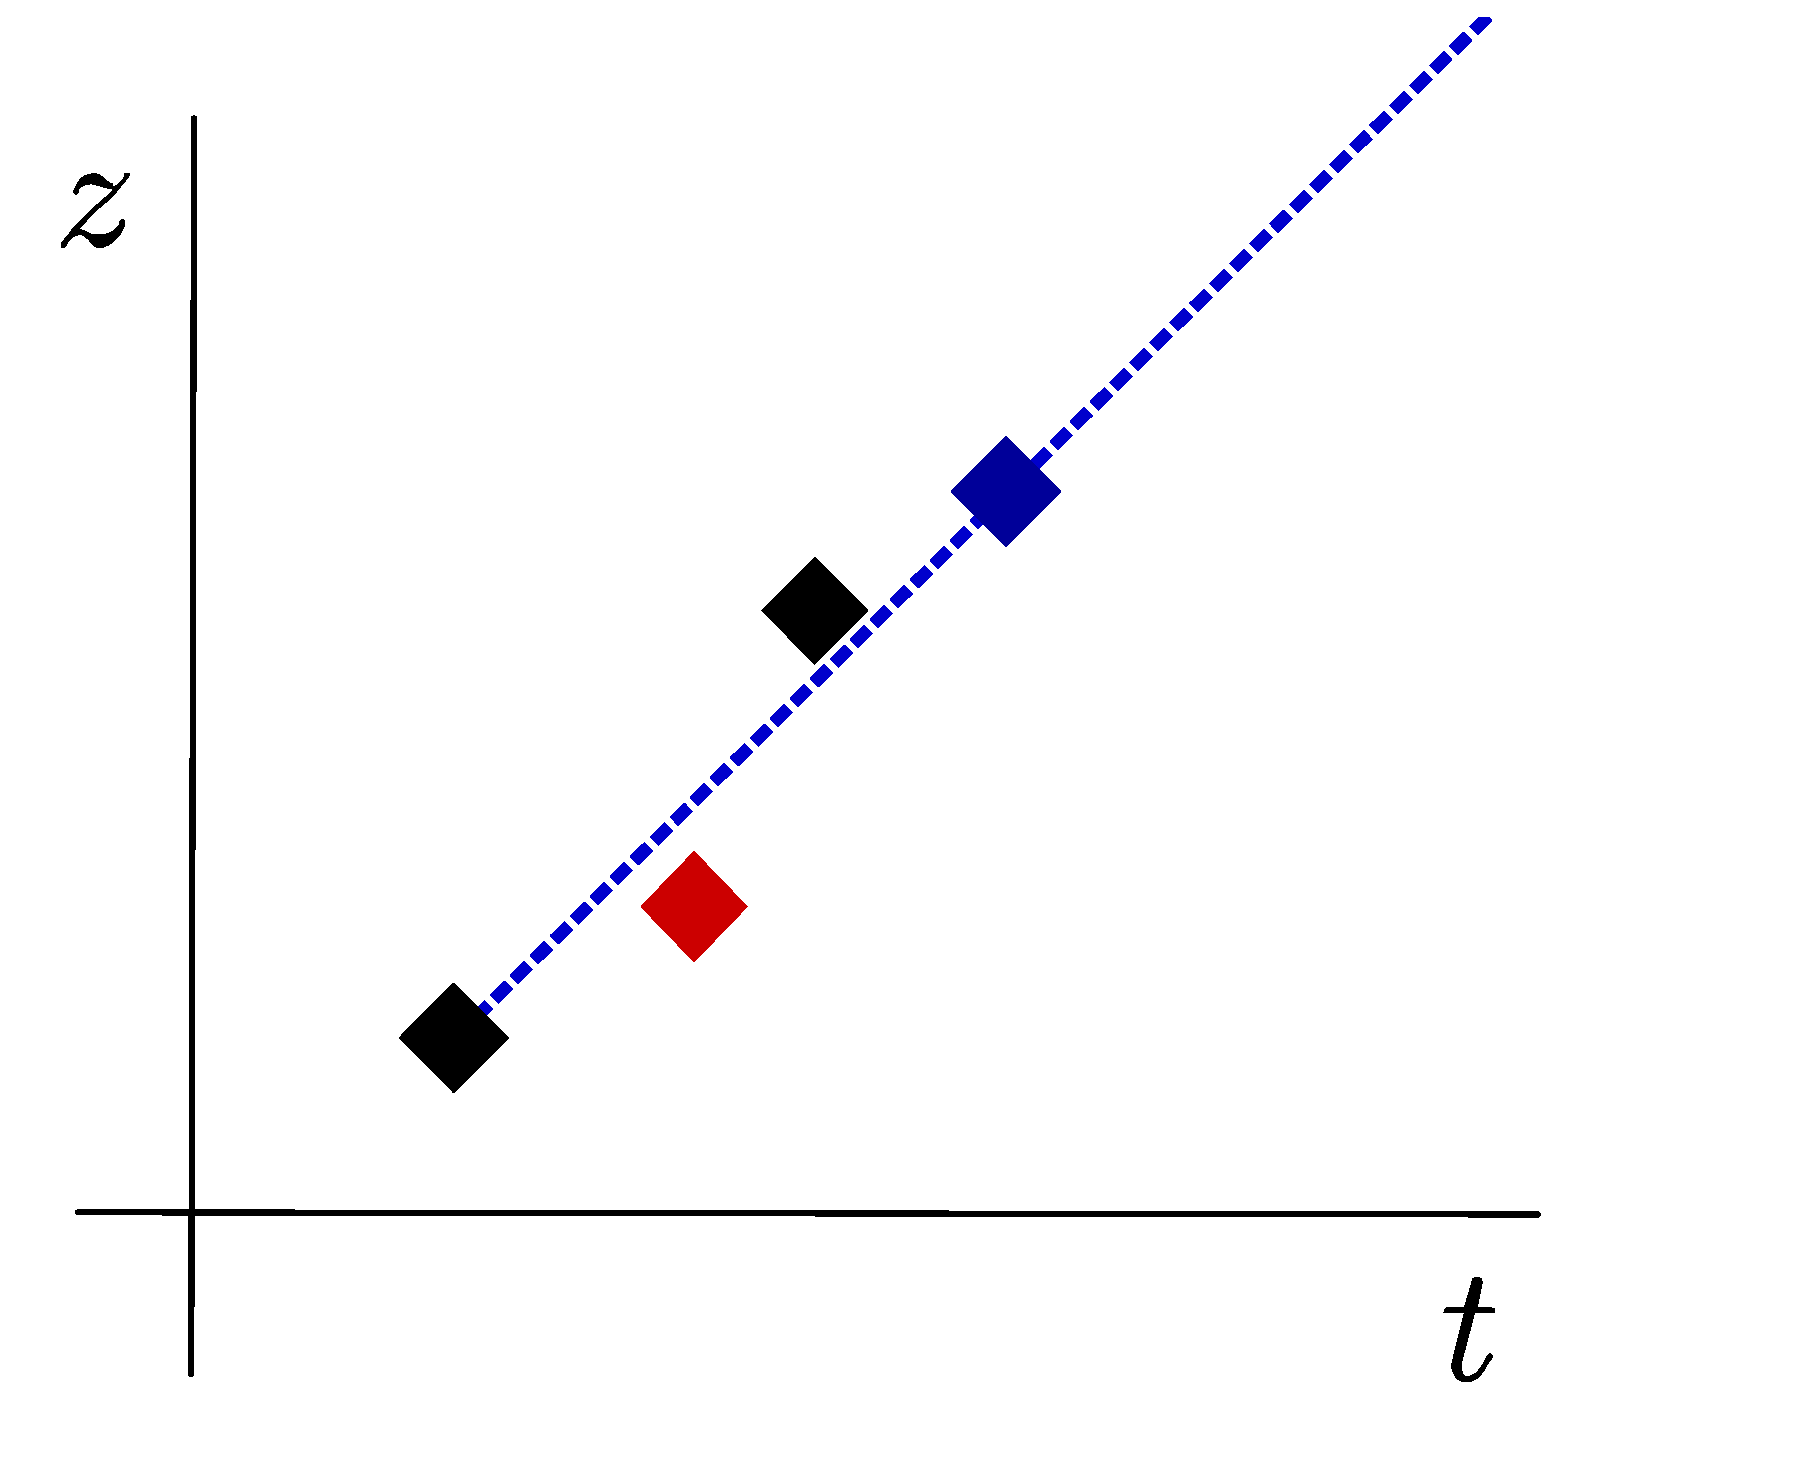
\includegraphics[width=0.37\textwidth]{selection4}
  \caption[Rejection of late pulses]{The latest pulse accepted (blue) is used to test if all previously ones selected still match the hypothesis. The pulse marked in red is discarded.}
  \label{fig:hit_discarded}
\end{figure}

\item The search continues until either the string ends, or 8 consecutive DOMs are found that either have no signal or are rejected.
\item Steps 5 through 8 are repeated but now for DOMs below DOM$_0$.
\item If three or more DOMs are found to match the conditions in one string, they are identified as containing direct pulses. In any other case, all of the pulses from the string are discarded.
\item Steps 1 through 10 are repeated until all strings have been scanned.
\end{enumerate}
Figure \ref{fig:good_selection} shows, for a simulated event, the steps that the algorithm takes in order to identify the direct photons. The dashed line corresponds to the expectation from pure Cherenkov light. Note that many pulses are removed, but the remaining ones follow the hyperbolic pattern.

\begin{figure}[tbh]
  \centering
  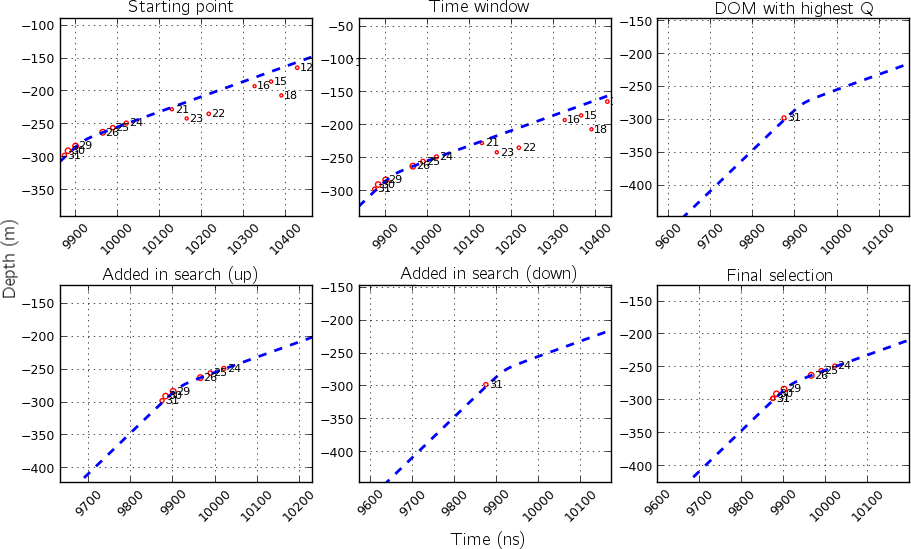
\includegraphics[width=0.9\textwidth]{santa_selection_good2}
  \caption[Step-wise example of the selection of direct pulses.]{Step-wise demonstration of the selection of direct pulses for one string of a simulated event. The expected alignment of the pulses is given by the blue dashed line. The number corresponds to the DOM position on the string, where 60 is the bottom-most one.}
  \label{fig:good_selection}
\end{figure}

The signals in the DOMs selected are assumed to be direct photons. The number of direct photons is used to judge the quality of the event, and can also be used to reconstruct the direction and position of muon tracks, as described in the following Section.




\textbf{[NOTE: we need plots for neutrinos and cosmic muons for all of these things]}
\\
\textbf{[Verify that all the variables used in LEESARD, DRAGON \& GRECO are listed]}




\end{document}
